\subsection{Εξέλιξη των μετρικών}

Στην ενότητα αυτή παρουσιάζεται η εξέλιξη των μετρικών στο χρόνο και
κατά τη διάρκεια των τριών sprint. Σε όλα τα γραφήματα, ο οριζόντιος
άξονας αναφέρεται στον αύξοντα αριθμό commit, ανάλογα με το χρόνο που
αυτό πραγματοποιήθηκε και ο κάθετος άξονας αναφέρεται στην τιμή της
μετρικής που εξετάζεται κάθε φορά.

\subsubsection{Logical Lines Of Code (LLOC)}
\label{section:projectLLOC}

Στο σχήμα \ref{fig:projectLLOC} εμφανίζεται η εξέλιξη του συνολικού
πλήθους των λογικών γραμμών κώδικα για το έργο. Παρατηρούμε ότι η
καμπύλη που απεικονίζει την μετρική LLOC, αυξάνεται σχεδόν γραμμικά σε
σχέση με τα commits. Το sprint 1, το οποίο αφορούσε στην ανάπτυξη της
backend λειτουργικότητας, ήταν το μικρότερο τόσο σε αριθμό γραμμών
κώδικα, όσο και σε διάρκεια (πλήθος commits). Τα περισσότερα commits
πραγματοποιήθηκαν στο sprint 2, όπου αναπτύχθηκε το μεγαλύτερο μέρος της
γραφικής διασύνδεσης της εφαρμογής. Οι περισσότερες γραμμές κώδικα όμως
προστέθηκαν κατά τη διάρκεια του sprint 3, αφού όπως είναι εμφανές και
στο γράφημα, κατά τη διάρκεια του sprint 3 υπήρξαν κάποια commits με τα
οποία προστέθηκαν αρκετές γραμμές κώδικα. Οι λόγοι που συνέβη αυτό ήταν
ότι τα μέλη της ομάδας είχαν πια εξοικειωθεί σε μεγάλο βαθμό με τη
μεθοδολογία ανάπτυξης της γραφικής διασύνδεσης και ότι κατά τη διάρκεια
του sprint 3, προστέθηκαν τα παράθυρα που αφορούσαν στη διαχείριση των
δωματίων και των τύπων δωματίων του ξενοδοχείου. Αυτά, σε αρκετά μεγάλο
βαθμό, λειτουργικά δανείζονται πολλά χαρακτηριστικά από τα αντίστοιχα
παράθυρα για τη διαχείριση των πελατών και των κρατήσεων που είχαν
αναπτυχθεί κατά τη διάρκεια του sprint 2.

\begin{figure}
\centering
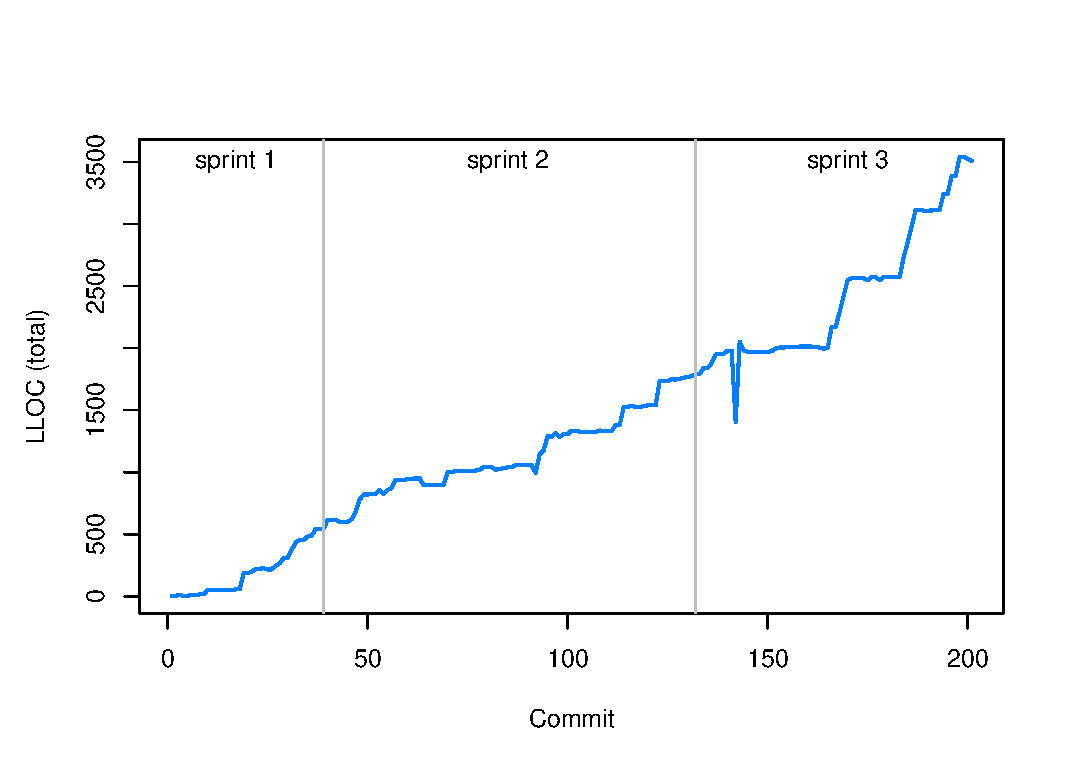
\includegraphics[width=1.0\textwidth]{Project-LLOC-1.eps}
\caption{Η μεταβολή των συνολικών λογικών γραμμών κώδικα (LLOC) στη διάρκεια της ανάπτυξης}
\label{fig:projectLLOC}
\end{figure}

Τόσο κατά τη διάρκεια του sprint 2, αλλά και του sprint 3,
υπήρξαν περιπτώσεις αρκετών διαδοχικών commits με τα οποία ο
αριθμός των γραμμών κώδικα που προστέθηκε στο έργο δεν αυξήθηκε.
Τα commits αυτά αφορούσαν κυρίως σε διορθώσεις προβλημάτων που
εντοπιζόταν κατά τη διάρκεια της ανάπτυξης.

Αξίζει να σημειωθεί ότι υπάρχει μια απότομη βύθιση της καμπύλης
κοντά στο 140ο commit με άμεση επαναφορά του αριθμού των γραμμών
κώδικα στην προηγούμενη τιμή τους. Αυτό οφείλεται σε commit που
έγινε εκτός της διακλάδωσης master στο αποθετήριο git, και σε
διακλάδωση η οποία δεν είχε συγχρονιστεί με αυτή πρόσφατα. Η
άμεση επαναφορά οφείλεται στη συγχώνευση της διακλάδωσης στη
διακλάδωση master που ακολούθησε. Όπως αναφέρθηκε προηγουμένως, ο
οριζόντιος άξονας του γραφήματος παρουσιάζει τα commits σε
χρονολογική σειρά. Η ανάπτυξη κώδικα όμως με τη χρήση
διακλαδώσεων, δεν είναι κατ’ ανάγκη γραμμική και ενδέχεται να
οδηγήσει σε περιπτώσεις όπως αυτή, όπου νέος κώδικας προστίθεται
σε μεταγενέστερο χρόνο σε κάποια μη ενημερωμένη διακλάδωση. Αν
και αυτό σε μεγάλο βαθμό αποφεύχθηκε στην παρούσα εργασία με τα
μέλη να συγχρονίζουν συχνά τις τοπικές τους διακλαδώσεις με τη
διακλάδωση master, στην περίπτωση αυτή συνέβη κάτι τέτοιο.

\subsubsection{Clone Coverage (CC)}

Στο σχήμα \ref{fig:projectCC} παρατηρούμε την εξέλιξη της μετρικής CC.
Βλέπουμε ότι λίγο πριν το τέλος του sprint 1 αυτή παρουσιάζει απότομη
αύξηση, δείγμα επαναχρησιμοποίησης κώδικα. Αυτό χρήζει διερεύνησης σε
επίπεδο κλάσης και όπως θα αναλυθεί περαιτέρω στην ενότητα
\ref{section:sprint1CC} όπου αναλύεται η τιμή της μετρικής
ανά κλάση στο τέλος του sprint 1, είναι τελικά σε ένα βαθμό
παραπλανητικό και τελικά δεν αποτελεί πρόβλημα.

\begin{figure}
\centering
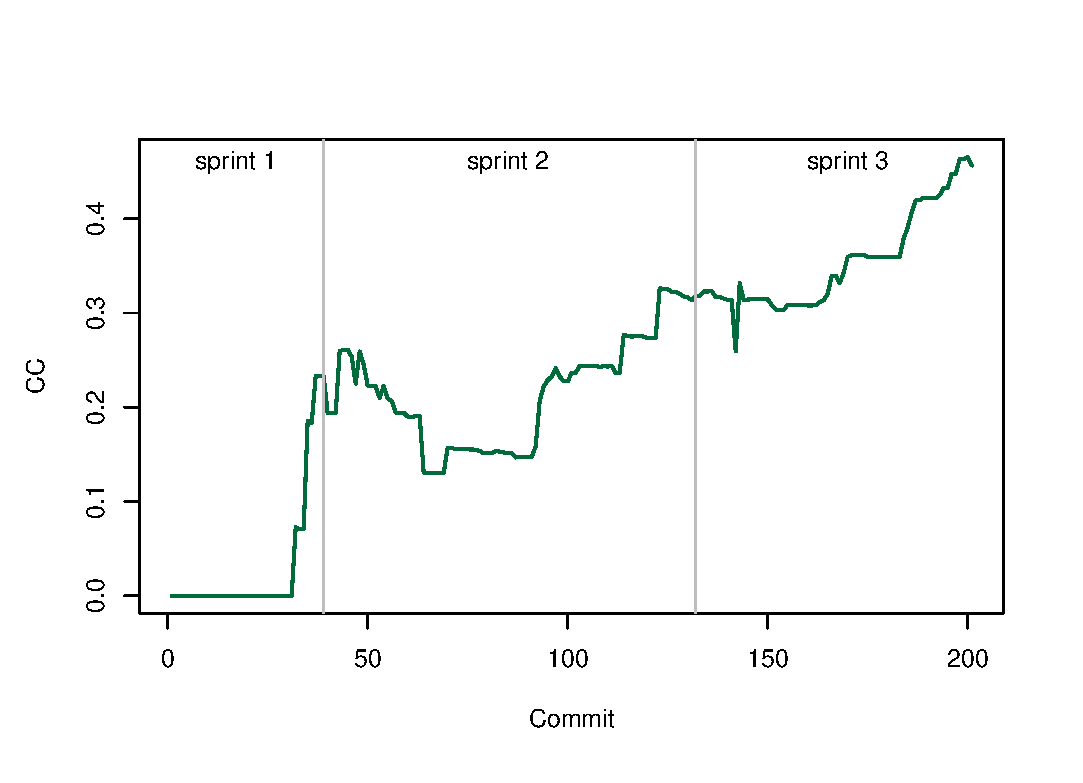
\includegraphics[width=1.0\textwidth]{Project-CC-1.eps}
\caption{Η εξέλιξη της μετρικής CC στη διάρκεια της ανάπτυξης}
\label{fig:projectCC}
\end{figure}

Η ακόλουθη πτώση των τιμών τις μετρικής στην αρχή του sprint 2 μέχρι
και τη μέση περίπου αυτού, δεν οφείλεται στη συνειδητή αντιμετώπιση
του προβλήματος από τα μέλη της ομάδας. Απλά, κατά τη διάρκεια του
sprint 2, προστέθηκε αρκετός νέος κώδικας, ο οποίος αφορούσε στη
γραφική διασύνδεση της εφαρμογής και δεν είχε κοινά χαρακτηριστικά
με τον κώδικα που αναπτύχθηκε κατά τη διάρκεια του sprint 1 ο οποίος
αφορούσε στο backend της εφαρμογής. Έτσι, με την αύξηση των
συνολικών γραμμών κώδικα, μειώθηκε το ποσοστό του επαναλαμβανόμενου
κώδικα.

Κατόπιν, παρατηρούμε ότι το ποσοστό επαναλαμβανόμενου κώδικα αυξάνει
σταδιακά, τόσο για το δεύτερο μισό του sprint 2, όσο και για το
sprint 3. Αυτό είναι σε ένα βαθμό αναμενόμενο, αφού οι διάφορες
κλάσεις γραφικής διασύνδεσης που σταδιακά προστέθηκαν στη διάρκεια
των δύο τελευταίων sprints έχουν αρκετά κοινά στοιχεία μεταξύ τους.
Για παράδειγμα, ο κώδικας διαχείρισης του κουμπιού κλεισίματος του
κάθε παραθύρου είναι τις περισσότερες φορές πανομοιότυπος για όλα τα
παράθυρα.

Η απότομη βύθιση και ανάκαμψη της καμπύλης κοντά στο 140ο commit
οφείλεται πάλι στην προσθήκη κώδικα σε μη πρόσφατα ενημερωμένη
διακλάδωση και την μετέπειτα συγχώνευση της διακλάδωσης στη
διακλάδωση master όπως αυτή περιγράφηκε αναλυτικότερα
στην ενότητα \ref{section:projectLLOC}

\subsubsection{McCabe's Cyclomatic Complexity (McCC)}

Η εξέλιξη της μέσης τιμής της μετρικής κυκλωματικής πολυπλοκότητας για
κάθε commit εμφανίζεται στο σχήμα \ref{fig:projectMcCC}. Αυτή υπολογίστηκε σε
επίπεδο κλάσης/enumeration και στη συνέχεια ως ο μέσος όρος των τιμών
κάθε κλάσης για κάθε commit. Παρατηρούμε ότι η κυκλωματική πολυπλοκότητα
παρουσιάζει συνεχή αύξηση. Αυτό συμβαίνει κυρίως λόγω της συνεχόμενης
προσθήκης λειτουργικότητας στο σύστημα. Αυτό είναι αναμενόμενο καθώς η
προσθήκη σύνθετων λειτουργιών απαιτεί χρήση δομών ελέγχου και επανάληψης
για να υλοποιηθούν. Στην αρχή του sprint 1 και στην αρχή του sprint 2
υπάρχει σημαντική πτώση της καμπύλης της μετρικής McCC, στις οποίες
παρουσιάζεται μείωση της συνολικής πολυπλοκότητας.

\begin{figure}
\centering
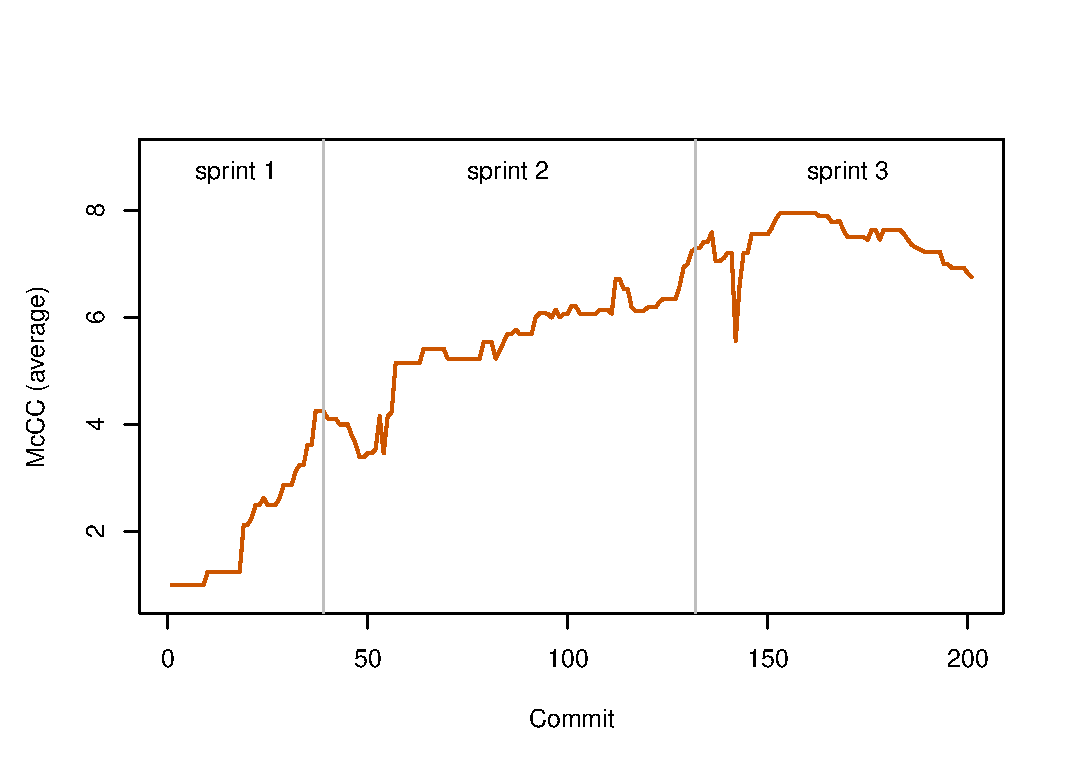
\includegraphics[width=1.0\textwidth]{Project-McCC-1.eps}
\caption{Η μεταβολή της μέσης τιμής της μετρικής κυκλωματικής
	πολυπλοκότητας (McCC) στη διάρκεια της ανάπτυξης}
\label{fig:projectMcCC}
\end{figure}

Η μέση τιμή της κυκλωματικής πολυπλοκότητας ακόμα και στο τέλος του
sprint 3 αξιολογείται ως ικανοποιητική. Λόγω του ότι πρόκειται για τη
μέση τιμή της μετρικής για τις κλάσεις, πιθανόν κάποιες κλάσεις να έχουν
αρκετά υψηλές τιμές, ενώ άλλες μηδενικές. Θα γίνει περαιτέρω διερεύνηση
στις ενότητες ανάλυσης των τριών sprint ανά κλάση.

Η απότομη βύθιση και ανάκαμψη της καμπύλης κοντά στο 140ο commit
οφείλεται ακόμα μια φορά στην προσθήκη κώδικα σε μη πρόσφατα ενημερωμένη
διακλάδωση και την μετέπειτα συγχώνευση της διακλάδωσης στη διακλάδωση
master όπως αυτή περιγράφηκε αναλυτικότερα στην ενότητα
\ref{section:projectLLOC}.

\subsubsection{Lack of Cohesion in Methods 5 (LCOM5)}

Στο σχήμα \ref{fig:projectLCOM5} εμφανίζεται η μεταβολή της μέσης τιμής
της μετρικής έλλειψης συνεκτικότητας LCOM5. Παρατηρούμε ότι αυτή
παρουσιάζει αυξητική τάση, με μία όμως λογική κλίση, πλην
του sprint 1, όπου έχουμε απότομες μεταβολές. Οι μεταβολές αυτές
οφείλονται στο σχετικά μικρό ακόμα μέγεθος του κώδικα και τις συχνές
αλλαγές στη δομή του με τη μεταφορά της βασικής λειτουργικότητας μεταξύ
των υπαρχόντων κλάσεων. Οι τιμές γενικά κυμαίνονται
σε χαμηλά επίπεδα, οπότε δεν αποτελούν σε αυτό το σημείο αντικείμενο
ανησυχίας.

\begin{figure}
\centering
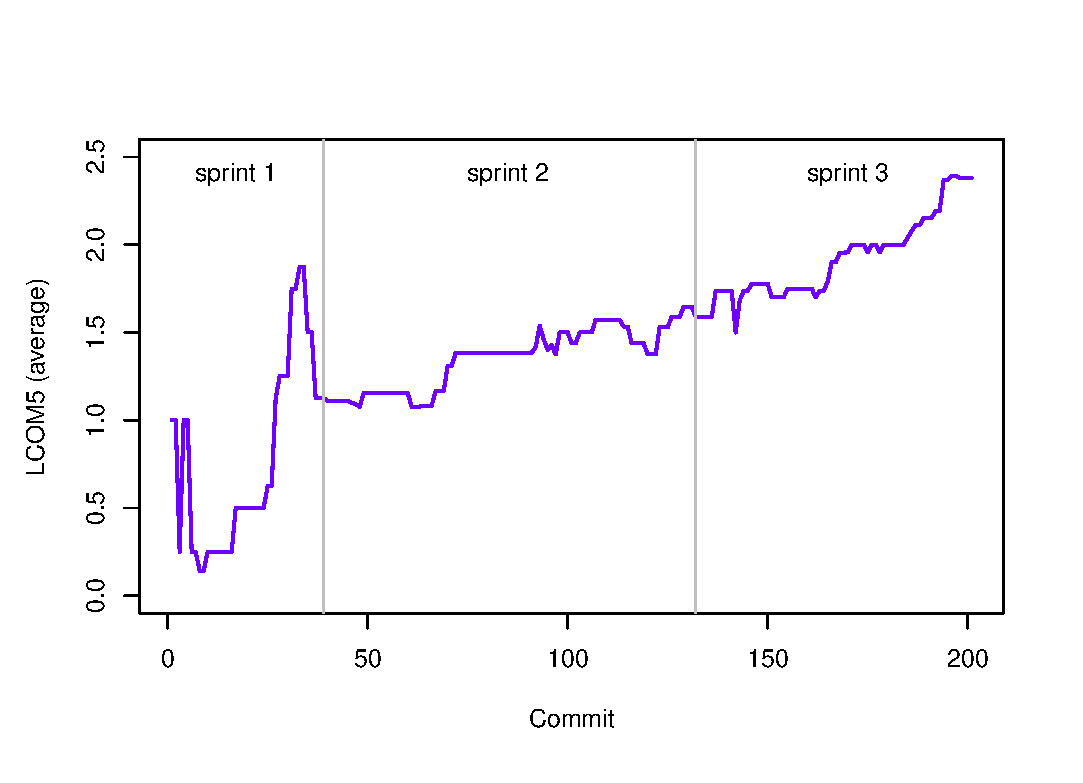
\includegraphics[width=1.0\textwidth]{Project-LCOM5-1.eps}
\caption{Η μεταβολή της μέσης τιμής της μετρικής έλλειψης συνοχής
LCOM5 στη διάρκεια της ανάπτυξης}
\label{fig:projectLCOM5}
\end{figure}

Γενικά δεν φαίνεται να καταστρατηγείται η αρχή της Μοναδικής
Αρμοδιότητας. Παρατηρούμε μεγάλη σχετικά αύξηση της μετρικής προς το τέλος του
sprint 3.
Στο σχήμα εμφανίζεται η μέση τιμή της μετρικής, το
οποίο σημαίνει ότι πιθανόν κάποιες κλάσεις έχουν χαμηλές τιμές και
κάποιες άλλες (ενδεχομένως λιγότερες) έχουν σχετικά αρκετά υψηλές τιμές.
Στο σημείο αυτό προστέθηκε κλάση για τη διαχείριση των
τύπων των δωματίων και πιθανόν σε αυτή να οφείλεται η αύξηση των τιμών.
Αυτό θα διερευνηθεί περαιτέρω στην ενότητα
\ref{section:sprint3LCOM5}.

\subsubsection{Coupling Between Object classes (CBO)}

Στο σχήμα \ref{fig:projectCBO} εμφανίζεται η μεταβολή της μέσης τιμής της
μετρικής σύζευξης CBO. Παρατηρούμε ότι η σύζευξη ανεβαίνει σε σχετικά υψηλά επίπεδα
(CBO>4), λαμβάνοντας υπόψη το σχετικά μικρό μέγεθος του συστήματος
(29 κλάσεις). Η καμπύλη αυξάνει και αυτό είναι αναμενόμενο, γιατί όσο
προστίθενται κλάσεις, τόσο αυξάνεται και το πλήθος των συνολικών
εξαρτήσεων του συστήματος.

\begin{figure}
\centering
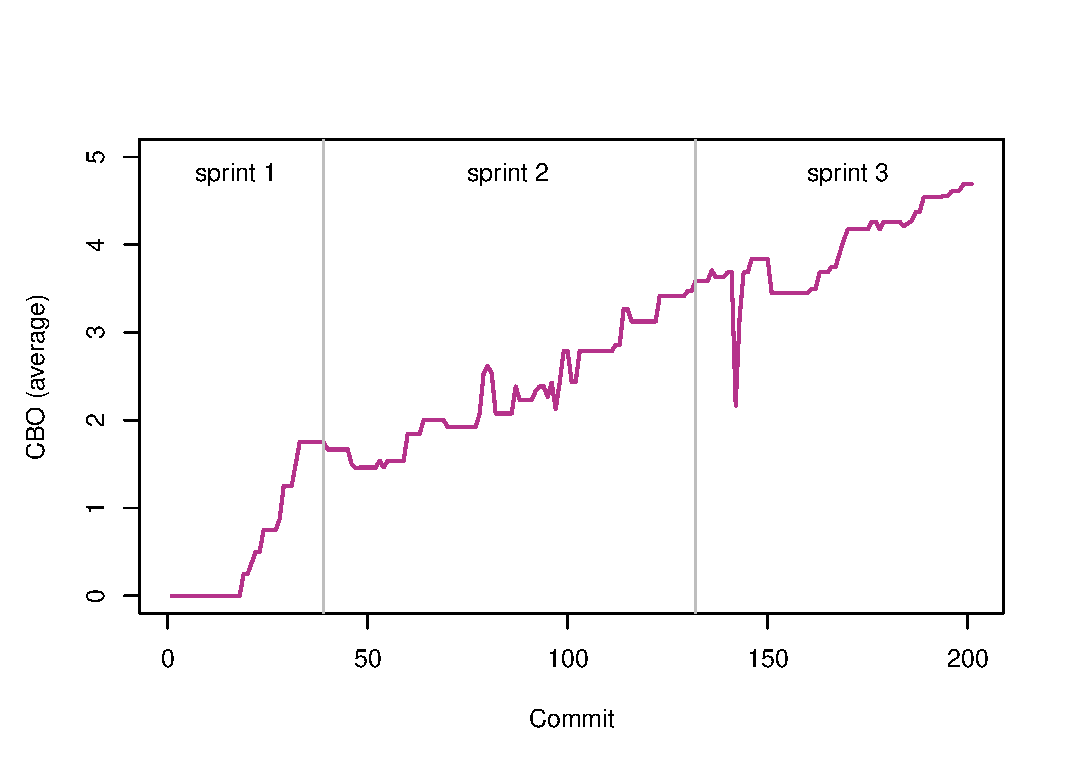
\includegraphics[width=1.0\textwidth]{Project-CBO-1.eps}
\caption{Η μεταβολή της μέσης τιμής της μετρικής σύζευξης
CBO στη διάρκεια της ανάπτυξης}
\label{fig:projectCBO}
\end{figure}

Η απότομη βύθιση της τιμής της μετρικής κοντά στο 140ο commit, οφείλεται
ακόμα μία φορά σε commit που έγινε σε μη ενημερωμένη διακλάδωση του
κώδικα όπως αναλύθηκε εκτενέστερα στην ενότητα \ref{section:projectLLOC}.

Καθότι υπολογίστηκε πάλι η μέση τιμή της μετρικής, η διαφορετική επιρροή
που έχουν οι κλάσεις μεμονωμένα στη διαμόρφωση της τιμής της μετρικής θα
εξεταστεί στις ενότητες \ref{section:sprint1CBO},
\ref{section:sprint2CBO} και \ref{section:sprint3CBO} αντίστοιχα για το
τέλος των τριών sprint.

